\chapter{Organização dos Sistemas Nervosos}\label{ch:b3:nervous-systems}

Uma água-viva tem alguns milhares de neurônios numa rede sem centro e
consegue nadar, se alimentar e se endireitar. Um polvo tem meio bilhão,
dois terços deles nos braços, cada um dos quais capaz de resolver um
problema de que o cérebro nem foi avisado. Você tem oitenta e seis
bilhões, unidos por cem trilhões de sinapses, funcionando com vinte
watts --- um quinto da sua energia para dois por cento da sua massa ---
e Santiago Ramón y Cajal, desenhando-os célula a célula na década de
1890 a partir de cortes corados pela prata, viu que eram células
separadas que se tocavam sem se fundir e que os sinais fluíam por elas
numa só direção. O volume anterior tratou do neurônio: seu potencial de
repouso, seu potencial de ação, sua sinapse. Este capítulo trata daquilo
em que os neurônios estão ligados: o cabo passivo que limita até onde um
sinal se espalha e com que rapidez, os circuitos --- reflexo, oscilador,
entorno inibitório --- com que o comportamento é montado, o plano do
sistema nervoso dos vertebrados e da \omterm{def:b3:nervous-systems:cells}{glia} que o mantém em
funcionamento, seu orçamento energético e os modos como diferentes
animais distribuíram seus neurônios.

\section{Neurônios e glia}

\begin{definition}[As células do sistema nervoso]\label{def:b3:nervous-systems:cells}
\index{neurônio!tipos}\index{glia}\index{astrócito}\index{oligodendrócito}\index{mielina}\index{micróglia}\index{interneurônio}
Os neurônios vêm em algumas poucas arquiteturas que se repetem por todo
o encéfalo: as células \emph{piramidais}, os neurônios excitatórios de
projeção do córtex, com um longo dendrito apical e um axônio que pode
percorrer um metro; as células de \emph{Purkinje} do \omterm{def:b3:nervous-systems:plan}{cerebelo}, cuja
árvore dendrítica achatada recebe duzentas mil sinapses; os neurônios
sensoriais, com um prolongamento para a periferia e outro para a
medula; e os \emph{interneurônios}, células de axônio curto que
permanecem dentro de uma região, a maioria delas inibitória. Cerca de
quatro em cada cinco neurônios corticais liberam glutamato e excitam;
um em cada cinco libera GABA e inibe. A \emph{glia}, tão numerosa
quanto os neurônios, faz o resto. Os \emph{astrócitos} envolvem sinapses
e vasos sanguíneos: captam o potássio que os neurônios em disparo
liberam e o glutamato que as sinapses derramam, fornecem lactato,
regulam localmente o fluxo sanguíneo e induzem e mantêm a \omterm{prop:b3:nervous-systems:barrier-budget}{barreira
hematoencefálica}. Os \emph{oligodendrócitos}, no sistema nervoso
central, e as \emph{células de Schwann}, na periferia, envolvem os
axônios em \emph{mielina}, dezenas de camadas de membrana que isolam o
axônio entre os nodos onde ficam os canais. A \emph{micróglia} são os
\omterm{def:b3:innate-immunity:innate}{macrófagos} residentes do encéfalo, que podam sinapses no
desenvolvimento e removem detritos. As células ependimárias revestem os
ventrículos e fazem o \omterm{prop:b3:nervous-systems:barrier-budget}{líquido cefalorraquidiano}.
\end{definition}

\begin{proof}[Evidência]
A coloração pelo cromato de prata de Golgi (1873) enegrecia, por razões
desconhecidas, cerca de um neurônio em cada cem, por inteiro, deixando
os demais invisíveis --- de modo que uma única célula podia ser vista
completa num emaranhado de milhões. Golgi leu suas próprias preparações
como um retículo contínuo; Cajal, a partir de 1888, usando a mesma
coloração em tecido embrionário, onde as células são mais simples, viu
que cada célula terminava livremente, que dendritos e axônio diferiam, e
que os axônios terminavam sobre os dendritos e os corpos de outras
células sem se unir a elas. Do arranjo das células sensoriais e motoras
inferiu a direção do fluxo --- do dendrito ao corpo e ao axônio ---, a
\emph{lei da polarização dinâmica}. Sherrington batizou a lacuna de
\emph{sinapse} em 1897; o microscópio eletrônico a mostrou em 1954.
\end{proof}

\begin{omfigure}
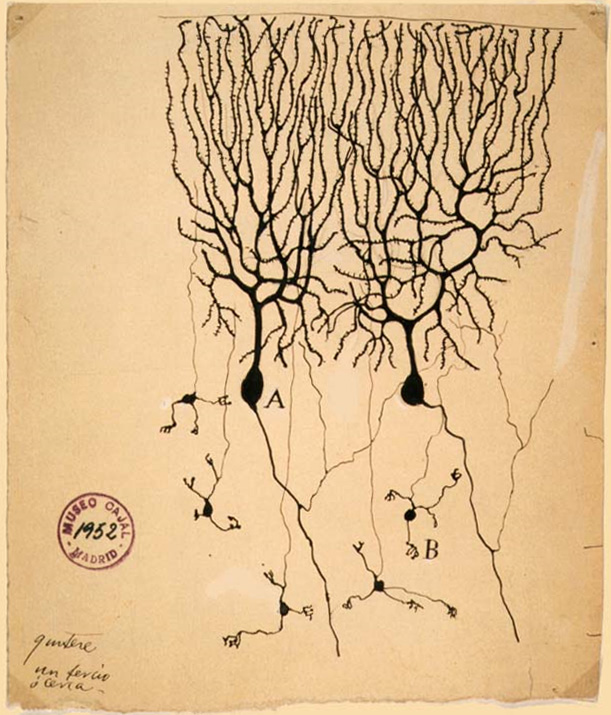
\includegraphics[width=0.30\linewidth]{images/book5/cajal-purkinje.jpg}\hspace{0.04\linewidth}
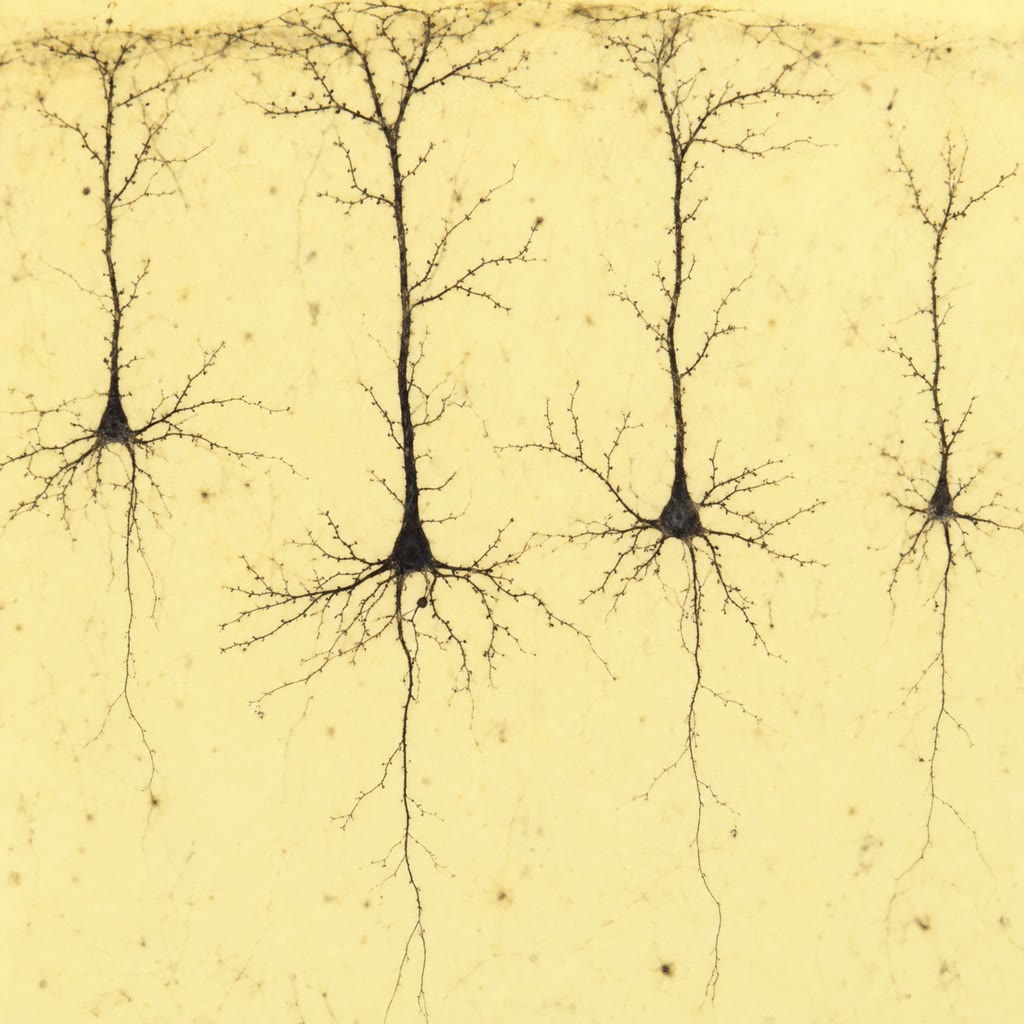
\includegraphics[width=0.30\linewidth]{images/book5/ai/b5-17-cortex-neurons.jpg}\hspace{0.04\linewidth}
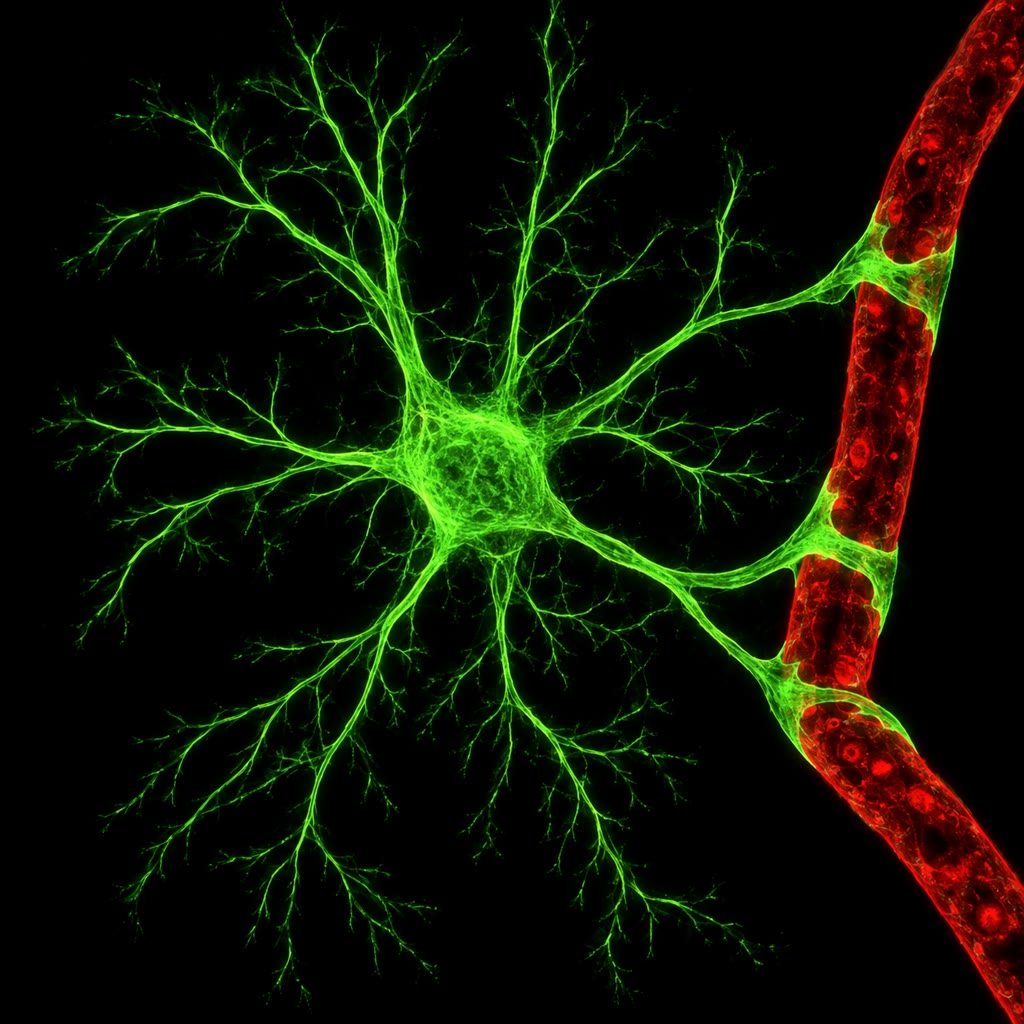
\includegraphics[width=0.30\linewidth]{images/book5/ai/b5-17-astrocyte.jpg}

{\small À esquerda: uma célula de Purkinje do \omterm{def:b3:nervous-systems:plan}{cerebelo} desenhada por
Cajal (1899) a partir de um corte corado por Golgi --- toda a árvore
dendrítica de uma célula, o argumento a favor do neurônio como unidade
(domínio público). No centro: neurônios piramidais do córtex numa
coloração de Golgi. À direita: um \omterm{def:b3:nervous-systems:cells}{astrócito} (verde) com seus pés
terminais sobre um capilar (vermelho).}
\end{omfigure}

\section{O neurônio como cabo}

\begin{theorem}[A equação do cabo em regime estacionário]\label{thm:b3:nervous-systems:cable}
\index{equação do cabo}\index{constante de comprimento}\index{constante de tempo!de membrana}\index{velocidade de condução}
Modele um dendrito ou um axônio amielínico como um cilindro de diâmetro
$d$ cujo citoplasma tem resistividade $R_{i}$ e cuja membrana tem
resistência específica $R_{m}$ (resistência vezes área) e capacitância
$C_{m}$ por área. Por unidade de comprimento, a resistência axial é
$r_{i} = 4R_{i}/\pi d^{2}$ e a resistência de membrana, $r_{m} = R_{m}/\pi d$. Uma voltagem estacionária $V_{0}$ aplicada em $x = 0$ se
espalha pela fibra como
\[
V(x) = V_{0}\,e^{-x/\lambda}, \qquad
\lambda = \sqrt{\frac{r_{m}}{r_{i}}} = \sqrt{\frac{R_{m}\,d}{4R_{i}}},
\]
onde $\lambda$ é a \emph{\omterm{thm:b3:nervous-systems:cable}{constante de comprimento}}: a distância ao longo
da qual um sinal passivo cai a $1/e$, crescendo com a raiz quadrada do
diâmetro. A membrana se carrega com a \emph{constante de tempo} $\tau =
R_{m}C_{m}$, independente da geometria. Um potencial de ação, que se
regenera, percorre um axônio amielínico a uma velocidade proporcional a
$\lambda/\tau$ e, portanto, a $\sqrt{d}$; ao longo de um axônio
mielínico, onde salta de nodo em nodo, a uma velocidade proporcional a
$d$ --- cerca de \qty{6}{m/s} por micrômetro de diâmetro.
\end{theorem}
\begin{proof}
Seja $I(x)$ a corrente axial. A lei de Ohm ao longo do núcleo dá
$\mathrm{d}V/\mathrm{d}x = -r_{i}I$; a conservação de carga em regime
estacionário diz que a corrente axial perdida entre $x$ e $x + \mathrm{d}x$ vaza pela membrana, $\mathrm{d}I/\mathrm{d}x = -V/r_{m}$.
Derivando a primeira e substituindo a segunda,
$\mathrm{d}^{2}V/\mathrm{d}x^{2} = (r_{i}/r_{m})V = V/\lambda^{2}$, uma
equação linear de segunda ordem cuja solução limitada quando $x \to \infty$ é $V_{0}e^{-x/\lambda}$. Substituindo $r_{m} = R_{m}/\pi d$ e
$r_{i} =
4R_{i}/\pi d^{2}$ obtém-se $\lambda^{2} = R_{m}d/4R_{i}$. A
constante de tempo é a de um resistor e um capacitor em paralelo,
$r_{m}c_{m} =
(R_{m}/\pi d)(C_{m}\pi d) = R_{m}C_{m}$. Quanto às
velocidades: uma onda que se regenera precisa carregar a membrana uma
\omterm{thm:b3:nervous-systems:cable}{constante de comprimento} à frente em cerca de uma constante de tempo, de
modo que $v \sim \lambda/\tau \propto \sqrt{d}$; entre os nodos de um
axônio mielínico a membrana internodal tem a resistência elevada e a
capacitância reduzida pela centena de camadas de \omterm{def:b3:nervous-systems:cells}{mielina}, o comprimento
do internodo escala com $d$, e o resultado é $v \propto d$. As
constantes de proporcionalidade são admitidas.
\end{proof}

\begin{example}[Números para um dendrito e dois axônios]\label{ex:b3:nervous-systems:numbers}
Um dendrito de $d = \qty{2}{\micro m}$ com $R_{m} = \qty{2e4}{\ohm.cm^2}$
e $R_{i} = \qty{100}{\ohm.cm}$: $\lambda = \sqrt{2\times 10^{4}\times
2\times 10^{-4}/400}\ \unit{cm} = \qty{0.1}{cm} = \qty{1}{mm}$ --- um
potencial sináptico na ponta de um dendrito de um milímetro chega ao
corpo celular com um terço do seu tamanho, e é por isso que a geometria
de uma árvore dendrítica faz parte do que ela computa. $\tau = 2\times 10^{4}\times
10^{-6}\,\unit{F/cm^2}\cdot\unit{\ohm.cm^2} = \qty{20}{ms}$,
a janela dentro da qual as entradas precisam chegar para se somar. Um
axônio gigante de lula de \qty{500}{\micro m}, amielínico, conduz a
cerca de \qty{25}{m/s}; para fazer o mesmo um vertebrado usa um axônio
mielínico de \qty{4}{\micro m}, quinze mil vezes menor em seção
transversal --- a razão pela qual um nervo de vertebrado pode carregar
dez mil fibras rápidas no espaço de um axônio de lula. Um axônio motor
de \qty{20}{\micro m} conduz a \qty{120}{m/s}; quando a esclerose
múltipla lhe arranca a \omterm{def:b3:nervous-systems:cells}{mielina}, a velocidade cai dez vezes e a condução
pode falhar por completo nos trechos desnudos.
\end{example}

\begin{omfigure}
\begin{tikzpicture}
\begin{axis}[
  width=6.4cm, height=5.2cm,
  axis x line=bottom, axis y line=left,
  xmin=0, xmax=3, ymin=0, ymax=1.05,
  xlabel={distância (mm)}, ylabel={$V/V_{0}$},
  xlabel style={font=\small, at={(axis description cs:0.5,-0.12)}, anchor=north}, ylabel style={font=\small},
  tick label style={font=\scriptsize}, xtick={0,1,2,3}, ytick={0,0.37,1}, yticklabels={0,$1/e$,1},
  clip=false,
]
\addplot[very thick, omDef, domain=0:3, samples=60] {exp(-x/1.0)};
\addplot[very thick, omThm, domain=0:3, samples=60] {exp(-x/0.5)};
\node[font=\scriptsize, omDef, anchor=south west] at (axis cs:1.2,0.45) {$d = \qty{2}{\micro m}$, $\lambda = \qty{1}{mm}$};
\node[font=\scriptsize, omThm, anchor=north west] at (axis cs:0.8,0.22) {$d = \qty{0.5}{\micro m}$, $\lambda = \qty{0.5}{mm}$};
\end{axis}
\begin{axis}[
  at={(7.6cm,0)}, anchor=south west,
  width=6.4cm, height=5.2cm,
  xmode=log, ymode=log,
  xmin=0.1, xmax=1000, ymin=0.1, ymax=200,
  xlabel={diâmetro do axônio ($\unit{\micro m}$)}, ylabel={velocidade (m/s)},
  xlabel style={font=\small, at={(axis description cs:0.5,-0.12)}, anchor=north}, ylabel style={font=\small},
  tick label style={font=\scriptsize},
  clip=false,
]
\addplot[very thick, omDef, domain=1:25, samples=2] {6*x};
\addplot[very thick, omThm, domain=0.2:1000, samples=2] {1.1*sqrt(x)};
\fill[omThm] (axis cs:500,25) circle (2pt); \node[font=\scriptsize, anchor=north east] at (axis cs:500,23) {axônio gigante de lula};
\fill[omDef] (axis cs:20,120) circle (2pt); \node[font=\scriptsize, anchor=west] at (axis cs:26,120) {axônio motor humano};
\node[font=\scriptsize, omDef, anchor=north west, align=left] at (axis cs:1.2,60) {mielínico: $v \propto d$};
\node[font=\scriptsize, omThm, anchor=north west, align=left] at (axis cs:2,0.7) {amielínico: $v \propto \sqrt{d}$};
\end{axis}
\end{tikzpicture}

{\small À esquerda: decaimento passivo de um sinal estacionário ao longo
de um dendrito, para dois diâmetros --- a \omterm{thm:b3:nervous-systems:cable}{constante de comprimento}
cresce com $\sqrt{d}$. À direita: \omterm{thm:b3:nervous-systems:cable}{velocidade de condução} em função do
diâmetro; a \omterm{def:b3:nervous-systems:cells}{mielina} permite que uma fibra de \qty{4}{\micro m} faça o
que um axônio amielínico precisa de meio milímetro para fazer.}
\end{omfigure}

\section{Circuitos}

\begin{definition}[Circuitos elementares]\label{def:b3:nervous-systems:circuits}
\index{arco reflexo}\index{inibição recíproca}\index{inibição anterógrada}\index{inibição por retroalimentação}\index{convergência}\index{divergência}
Um \emph{arco reflexo} é o caminho mais curto de um sensor a um efetor:
no reflexo patelar, um aferente do fuso muscular entra na medula e faz
sinapse diretamente sobre os neurônios motores do mesmo músculo, que o
contraem cerca de \qty{30}{ms} depois da batida --- uma sinapse, sem
encéfalo. O mesmo aferente excita um \omterm{def:b3:nervous-systems:cells}{interneurônio} inibitório dirigido
aos neurônios motores do músculo oposto (\emph{inibição recíproca}),
para que a contração do extensor não seja combatida pelo flexor. A
maioria dos circuitos é construída a partir de alguns motivos: a
\emph{divergência}, um neurônio acionando muitos, e a
\emph{convergência}, muitos sobre um, que soma evidências; a
\emph{inibição anterógrada}, em que uma entrada excita ao mesmo tempo um
alvo e um \omterm{def:b3:nervous-systems:cells}{interneurônio} que inibe esse alvo um milissegundo depois,
afinando a resposta no tempo; a \emph{inibição por retroalimentação}, em
que a própria saída do alvo excita um \omterm{def:b3:nervous-systems:cells}{interneurônio} que o inibe,
limitando o disparo e, estendida aos vizinhos, produzindo a inibição
lateral que realça o contraste (\cref{ch:b3:sensory-systems}); e a
\emph{desinibição}, inibir um inibidor, o modo como os núcleos da base
liberam um movimento.
\end{definition}

\begin{omfigure}
\begin{tikzpicture}[every node/.style={font=\scriptsize}, >=stealth]
  % spinal cord cross-section (schematic)
  \draw[thick, omDef!60, fill=omDef!8] (5.4,1.5) ellipse (2.0 and 1.5);
  \draw[thick, gray, fill=gray!15] (5.4,1.5) .. controls (4.7,2.4) and (4.0,2.6) .. (4.0,1.9) .. controls (4.0,1.2) and (4.6,0.9) .. (4.8,0.5) .. controls (5.0,0.2) and (5.8,0.2) .. (6.0,0.5) .. controls (6.2,0.9) and (6.8,1.2) .. (6.8,1.9) .. controls (6.8,2.6) and (6.1,2.4) .. (5.4,1.5);
  \node[above] at (5.4,3.05) {medula espinal};
  % muscles
  \draw[thick, omMeth!70!black, fill=omMeth!20] (0.2,0.2) rectangle (1.4,2.0); \node[below, align=center] at (0.8,0.1) {extensor\\(quadríceps)};
  \draw[thick, omThm!70!black, fill=omThm!15] (0.2,-2.6) rectangle (1.4,-1.4); \node[below, align=center] at (0.8,-2.7) {flexor\\(isquiotibiais)};
  \fill[omProp] (0.8,1.3) ellipse (0.12 and 0.3); \node[left, font=\tiny] at (0.65,1.3) {fuso};
  % Ia afferent to cord (dorsal)
  \draw[very thick, omProp] (0.9,1.3) .. controls (2.0,2.6) and (3.6,2.9) .. (4.8,2.2); \fill[omProp] (4.8,2.2) circle (0.09);
  \node[above, omProp] at (2.6,2.85) {aferente Ia: estiramento};
  % motor neuron to extensor
  \fill[omMeth!70!black] (5.0,0.9) circle (0.16);
  \draw[->, very thick, omMeth!70!black] (4.9,0.85) .. controls (3.4,0.3) and (2.0,0.4) .. (1.4,1.0);
  \draw[->, thick, omProp] (4.8,2.2) -- (5.0,1.1);
  % inhibitory interneuron to flexor motor neuron
  \fill[omThm] (6.1,1.7) circle (0.13);
  \draw[->, thick, omProp] (4.9,2.25) -- (6.0,1.8);
  \fill[omThm!70!black] (6.0,0.6) circle (0.16);
  \draw[-|, thick, omThm] (6.1,1.55) -- (6.0,0.8);
  \draw[->, very thick, omThm!70!black, dashed] (5.9,0.5) .. controls (4.8,-0.8) and (3.0,-1.6) .. (1.4,-2.0);
  % right-hand labels with leaders
  \node[right, omThm, font=\tiny] at (7.6,1.9) {interneurônio inibitório Ia}; \draw[gray, thin] (7.55,1.9) -- (6.25,1.7);
  \node[right, omMeth!70!black, font=\tiny, align=left] at (7.6,1.1) {neurônio motor do extensor: excitado}; \draw[gray, thin] (7.55,1.1) -- (5.15,0.9);
  \node[right, omThm!70!black, font=\tiny, align=left] at (7.6,0.3) {neurônio motor do flexor: inibido}; \draw[gray, thin] (7.55,0.3) -- (6.15,0.6);
  \node[below] at (4.6,-0.15) {reflexo monossináptico: $\sim$\qty{30}{ms}};
  \node[below, align=center] at (4.2,-2.0) {inibição recíproca:\\o antagonista relaxa};
\end{tikzpicture}

{\small O reflexo de estiramento. Uma batida estira os fusos do
extensor; o aferente Ia excita diretamente os neurônios motores do
extensor (uma sinapse) e, através de um \omterm{def:b3:nervous-systems:cells}{interneurônio} inibitório,
silencia os do flexor.}
\end{omfigure}

\begin{proposition}[Geradores centrais de padrões]\label{prop:b3:nervous-systems:cpg}
\index{gerador central de padrões}\index{oscilador de meio-centro}
Os movimentos rítmicos --- respirar, andar, nadar, mastigar --- são
produzidos por circuitos do \omterm{def:b3:nervous-systems:plan}{tronco encefálico} e da \omterm{def:b3:nervous-systems:plan}{medula espinal} que
oscilam por conta própria, os \emph{geradores centrais de padrões}, que
a retroalimentação sensorial ajusta mas não cria: a \omterm{def:b3:nervous-systems:plan}{medula espinal} de um
gato separada do encéfalo e privada de seus nervos sensoriais ainda
produz o padrão alternado da marcha. O projeto mais simples é o
\emph{meio-centro} de Brown (1911): dois grupos de neurônios que se
inibem mutuamente. Aquele que disparar silencia o parceiro; mas um grupo
que dispara se cansa --- seus canais inativam, sua inibição do parceiro
enfraquece --- e o parceiro, liberado, dispara e, por sua vez, silencia
o primeiro: alternância, com um período fixado pela constante de tempo
do cansaço, e não por relógio algum. O ritmo respiratório nasce num
agrupamento de alguns milhares de neurônios do bulbo (o complexo
pré-Bötzinger), que dispara em salvas do nascimento à morte; a natação
da lampreia é uma cadeia de meio-centros ao longo de sua medula, cada
um atrasado em relação ao anterior, de modo que uma onda viaja rumo à
cauda.
\end{proposition}

\begin{omfigure}
\begin{tikzpicture}[every node/.style={font=\scriptsize}, >=stealth]
  % half-centre
  \begin{scope}
    \draw[thick, fill=omDef!25] (0,0) circle (0.5); \node at (0,0) {E};
    \draw[thick, fill=omThm!25] (3,0) circle (0.5); \node at (3,0) {D};
    \draw[-|, very thick] (0.5,0.2) -- (2.5,0.2); \draw[-|, very thick] (2.5,-0.2) -- (0.5,-0.2);
    \node[above] at (1.5,0.3) {inibição mútua};
    \draw[->, thick, omDef] (0,-0.5) -- (0,-1.3) node[below] {músculos esquerdos};
    \draw[->, thick, omThm] (3,-0.5) -- (3,-1.3) node[below] {músculos direitos};
    \draw[->, thick, gray] (-1.2,0.6) -- (-0.45,0.25) node[pos=0, above, align=center] {estímulo tônico\\do tronco encefálico};
    \draw[->, thick, gray] (4.5,0.6) -- (3.45,0.25);
  \end{scope}
  % traces
  \begin{scope}[xshift=6.0cm, yshift=0.9cm]
    \node[left, omDef] at (0,0) {E};
    \foreach \x in {0,2,4} { \foreach \s in {0.1,0.2,...,0.9} \draw[omDef] (\x+\s,-0.15) -- (\x+\s,0.15); }
    \node[left, omThm] at (0,-1.0) {D};
    \foreach \x in {1,3,5} { \foreach \s in {0.1,0.2,...,0.9} \draw[omThm] (\x+\s,-1.15) -- (\x+\s,-0.85); }
    \draw[->] (0,-1.6) -- (6.2,-1.6) node[right] {tempo};
    \draw[<->] (0,-2.0) -- (2,-2.0) node[midway, below] {período: fixado pelo cansaço};
  \end{scope}
\end{tikzpicture}

{\small Um \omterm{prop:b3:nervous-systems:cpg}{oscilador de meio-centro}. Dois grupos que se inibem
mutuamente, sob estímulo constante, alternam: o lado ativo se cansa, sua
inibição enfraquece, o outro lado escapa e assume. Nenhum neurônio é,
ele próprio, rítmico.}
\end{omfigure}

\begin{method}[Rastrear um circuito]\label{met:b3:nervous-systems:tracing}
\index{rastreamento de circuitos}\index{optogenética}
Para estabelecer que o neurônio A aciona o neurônio B e que a via
importa para um comportamento: (1) anatomia --- injete um traçador que
viaje pelos axônios (um corante, um \omterm{def:b3:virology:virus}{vírus} da raiva modificado que
atravessa uma sinapse para trás) e encontre as células conectadas; (2)
fisiologia --- registre de B enquanto estimula A, e meça a latência (uma
conexão monossináptica dá um atraso fixo de cerca de um milissegundo) e
o sinal (excitação ou inibição); (3) necessidade --- silencie A, por
lesão, por resfriamento ou expressando nele uma bomba de cloreto
acionada por luz e acendendo a luz (\emph{optogenética}), e veja se o
comportamento falha; (4) suficiência --- ative A sozinho, com um canal
de cátions acionado por luz, e veja se o comportamento aparece; (5) num
animal intacto, registre por imagem a atividade de toda a população com
um indicador de cálcio enquanto o comportamento é executado. Um circuito
está estabelecido quando os cinco concordam; a maioria dos circuitos
publicados tem dois ou três.
\end{method}

\section{O plano do sistema nervoso dos vertebrados}

\begin{definition}[Divisões central e periférica]\label{def:b3:nervous-systems:plan}
\index{medula espinal}\index{tronco encefálico}\index{cerebelo}\index{tálamo}\index{hipotálamo}\index{córtex cerebral}\index{sistema nervoso autônomo}\index{sistema nervoso entérico}
O \emph{sistema nervoso central} é o encéfalo e a medula espinal; o
\emph{periférico} é todo o resto. A \emph{medula espinal} recebe axônios
sensoriais pelas raízes dorsais e envia axônios motores pelas raízes
ventrais; sua substância cinzenta é uma borboleta de corpos celulares e
sua substância branca são os tratos mielinizados que sobem e descem. O
\emph{tronco encefálico} --- bulbo, ponte, mesencéfalo --- abriga os
núcleos dos nervos cranianos e os centros que mantêm a respiração, a
frequência cardíaca e a pressão arterial sem que se pense nisso; a morte
do tronco encefálico é a morte. O \emph{cerebelo}, com mais neurônios
que todo o resto do encéfalo, ajusta o tempo e a coordenação do
movimento e aprende com o erro. O \emph{tálamo} retransmite ao córtex
todos os sentidos exceto o olfato, e de volta as respostas do córtex; o
\emph{hipotálamo}, abaixo dele, comanda a homeostase --- temperatura,
fome, sede, o relógio, os eixos endócrinos do
\cref{ch:b3:endocrinology}. Os \emph{núcleos da base} selecionam entre
as ações possíveis; o \emph{hipocampo} fabrica memórias
(\cref{ch:b3:learning-memory}); e o \emph{córtex cerebral}, uma lâmina
de seis camadas de células com dois a quatro milímetros de espessura e
um quarto de metro quadrado de área, dobrada para caber, faz o resto, em
áreas mapeadas para cada sentido e cada movimento e em áreas de
associação entre elas. A divisão \emph{autônoma} do sistema periférico
comanda os órgãos: a cadeia \emph{simpática}, que libera noradrenalina,
mobiliza (coração acelerado, intestino parado, pupilas dilatadas); os
nervos \emph{parassimpáticos}, que liberam acetilcolina, poupam e
digerem; e o sistema nervoso \emph{entérico}, meio bilhão de neurônios
na parede do intestino, comanda a digestão por conta própria.
\end{definition}

\begin{omfigure}
\begin{tikzpicture}[every node/.style={font=\scriptsize}, >=stealth]
  % sagittal brain schematic
  \draw[thick, omDef!70, fill=omDef!15] (0,2.0) .. controls (0,4.6) and (3.5,5.4) .. (6.0,4.4) .. controls (7.6,3.7) and (7.4,2.2) .. (6.2,1.9) .. controls (5.4,1.7) and (5.2,1.3) .. (4.4,1.6) .. controls (3.0,1.3) and (1.2,1.4) .. (0,2.0);
  \node[align=center] at (3.0,3.9) {córtex cerebral: seis camadas,\\áreas sensoriais, motoras e de associação};
  % basal ganglia / hippocampus (deep)
  \draw[thick, omProp!70, fill=omProp!25] (3.2,2.6) ellipse (0.9 and 0.45); \node[font=\tiny] at (3.2,2.6) {núcleos da base};
  \draw[thick, omProp!70, fill=omProp!25] (5.2,2.45) ellipse (0.88 and 0.3); \node[font=\tiny] at (5.2,2.45) {hipocampo};
  % thalamus, hypothalamus
  \draw[thick, omMeth!70!black, fill=omMeth!25] (4.0,1.95) ellipse (0.7 and 0.3); \node[font=\tiny] at (4.0,1.95) {tálamo};
  \draw[thick, omMeth!70!black, fill=omMeth!40] (4.0,1.42) ellipse (0.78 and 0.22); \node[font=\tiny] at (4.0,1.42) {hipotálamo};
  % cerebellum
  \draw[thick, omThm!70, fill=omThm!20] (6.6,1.2) ellipse (0.9 and 0.6); \node[font=\tiny] at (6.6,1.2) {cerebelo};
  % brainstem
  \draw[thick, gray!70, fill=gray!20] (4.7,1.2) -- (5.5,1.2) -- (5.9,-0.3) -- (5.1,-0.3) -- cycle; \node[font=\tiny, rotate=-75] at (5.3,0.45) {tronco encefálico};
  % spinal cord
  \draw[thick, gray!70, fill=gray!20] (5.2,-0.3) rectangle (5.8,-1.6); \node[right, font=\tiny] at (5.85,-1.0) {medula espinal};
  % labels with leaders on the right
  \node[right, align=left] at (7.8,3.4) {tálamo: retransmissão de todos os\\sentidos menos o olfato; hipotálamo:\\homeostase, relógio, eixos endócrinos};
  \draw[gray] (7.75,3.3) -- (4.7,1.95);
  \node[right, align=left] at (7.8,1.9) {cerebelo: tempo e\\coordenação, aprendizado com o erro};
  \draw[gray] (7.75,1.8) -- (7.5,1.4);
  \node[right, align=left] at (7.8,0.4) {tronco encefálico: respiração, coração,\\nervos cranianos (bulbo,\\ponte, mesencéfalo)};
  \draw[gray] (7.75,0.4) -- (5.9,0.4);
  \node[right, align=left] at (7.8,-1.0) {medula espinal: reflexos, geradores\\de padrões, tratos que sobem e descem};
\end{tikzpicture}

{\small O encéfalo dos vertebrados em corte sagital, esquematicamente: o
córtex sobre os núcleos profundos, o \omterm{def:b3:nervous-systems:plan}{tálamo} e o \omterm{def:b3:nervous-systems:plan}{hipotálamo} no centro, o
\omterm{def:b3:nervous-systems:plan}{cerebelo} atrás, o \omterm{def:b3:nervous-systems:plan}{tronco encefálico} continuando na medula.}
\end{omfigure}

\begin{proposition}[A barreira hematoencefálica e o orçamento do encéfalo]\label{prop:b3:nervous-systems:barrier-budget}
\index{barreira hematoencefálica}\index{líquido cefalorraquidiano}\index{orçamento energético do encéfalo}
Os capilares do encéfalo são vedados por junções oclusivas entre suas
células endoteliais, envolvidos por pés terminais de \omterm{def:b3:nervous-systems:cells}{astrócitos} e
equipados com transportadores que admitem glicose e aminoácidos e
bombeiam para fora quase todo o resto: a \emph{\omterm{prop:b3:nervous-systems:barrier-budget}{barreira
hematoencefálica}}, que mantém constante a composição iônica do líquido
extracelular do encéfalo em nome do comportamento elétrico dos
neurônios, e que exclui a maioria dos fármacos (\qty{98}{\%} das
moléculas pequenas, todos os \omterm{def:b3:adaptive-immunity:antibody}{anticorpos}) --- o problema central da
neurofarmacologia. O encéfalo flutua em \qty{150}{mL} de \emph{\omterm{prop:b3:nervous-systems:barrier-budget}{líquido
cefalorraquidiano}}, produzido a meio mililitro por minuto e renovado
quatro vezes ao dia, que o amortece e leva embora os resíduos,
sobretudo durante o sono. O custo do encéfalo: uns \qty{20}{W} num
adulto, \qty{20}{\%} do metabolismo de repouso, quase tudo como glicose
queimada em ATP, e a maior parte desse ATP gasta pela bomba de sódio ao
restaurar os gradientes que os potenciais de ação e as correntes
sinápticas consomem. A \qty{50}{kJ} por mol de ATP, \qty{20}{W} são
$4\times 10^{-4}$ mol de ATP por segundo, $2.4\times 10^{20}$
moléculas; divididos entre $8.6\times 10^{10}$ neurônios, cerca de
$3\times 10^{9}$ ATP por neurônio por segundo. Um potencial de ação
cortical, com suas consequências sinápticas, custa da ordem de $10^{9}$
ATP, de modo que o orçamento permite uma frequência média de disparo de
alguns poucos potenciais por segundo por neurônio --- e os neurônios
corticais disparam mais ou menos a essa taxa. O encéfalo é construído
sob um limite energético estrito, e é por isso que seus sinais são
esparsos, seus axônios finos e sua informação codificada por poucos
disparos em muitas células.
\end{proposition}
\admitted

\section{Sistemas nervosos pelos animais afora}

\begin{definition}[Redes nervosas, gânglios e encéfalos]\label{def:b3:nervous-systems:comparative}
\index{rede nervosa}\index{gânglio}\index{cefalização}\index{encefalização}
Os cnidários (águas-vivas, hidras) têm uma \emph{rede nervosa}:
neurônios distribuídos pela parede do corpo, conectados em todas as
direções, com condensações em anel ao redor da margem do sino que
coordenam a natação --- nenhum centro, e condução nos dois sentidos ao
longo de cada célula. Os animais bilatérios concentram neurônios em
\emph{gânglios} --- agrupamentos com um neurópilo compartilhado ---
dispostos ao longo de um cordão ventral nos artrópodes e anelídeos, com
um gânglio cefálico aumentado onde estão os órgãos dos sentidos: a
\emph{cefalização}. Os moluscos variam dos gânglios simples de um
mexilhão ao polvo, cujo meio bilhão de neurônios é o maior de qualquer
invertebrado e dois terços do qual ficam nos braços, com o cordão de
cada braço controlando seu próprio alcançar e agarrar. Os vertebrados
constroem um tubo dorsal oco, expandido na frente no encéfalo da seção
anterior, protegido por osso e por uma barreira, e mielinizado. As
mesmas moléculas de sinalização, canais, transmissores e muitos dos
mesmos genes do desenvolvimento (o código Hox do rombencéfalo, os
fatores de padronização do olho) operam em todos eles: as peças são
antigas e compartilhadas, os arranjos, diversos.
\end{definition}

\begin{example}[Contar neurônios]\label{ex:b3:nervous-systems:counts}
Um nematódeo tem $302$ neurônios, cada um deles nomeado e cada sinapse
mapeada; uma mosca-das-frutas, $1.4\times 10^{5}$; uma abelha,
$10^{6}$; um camundongo, $7\times 10^{7}$; um polvo, $5\times 10^{8}$;
um humano, $8.6\times
10^{10}$; um elefante, $2.6\times 10^{11}$, a
maioria deles em seu \omterm{def:b3:nervous-systems:plan}{cerebelo}. A massa encefálica escala com a massa
corporal entre os mamíferos aproximadamente como $M_{\text{encéfalo}} \propto M_{\text{corpo}}^{0.75}$, de modo que o encéfalo de um camundongo
é uma fração maior de seu corpo que o de um elefante; as espécies acima
da linha para seu tamanho --- golfinhos, primatas, humanos por um fator
sete --- são ditas encefalizadas. O que melhor acompanha a cognição não
é a massa encefálica, mas o número de neurônios do \omterm{def:b3:nervous-systems:plan}{córtex cerebral}:
cerca de $1.6\times 10^{10}$ num humano, $5.6\times 10^{9}$ no elefante,
cujo encéfalo é três vezes maior, $2\times 10^{9}$ num chimpanzé. O
encéfalo humano não é especial em suas células nem em seu plano; ele tem
mais neurônios corticais que qualquer outro, empacotados mais
densamente, e é o número, e não o peso, que parece contar.
\end{example}

\begin{omfigure}
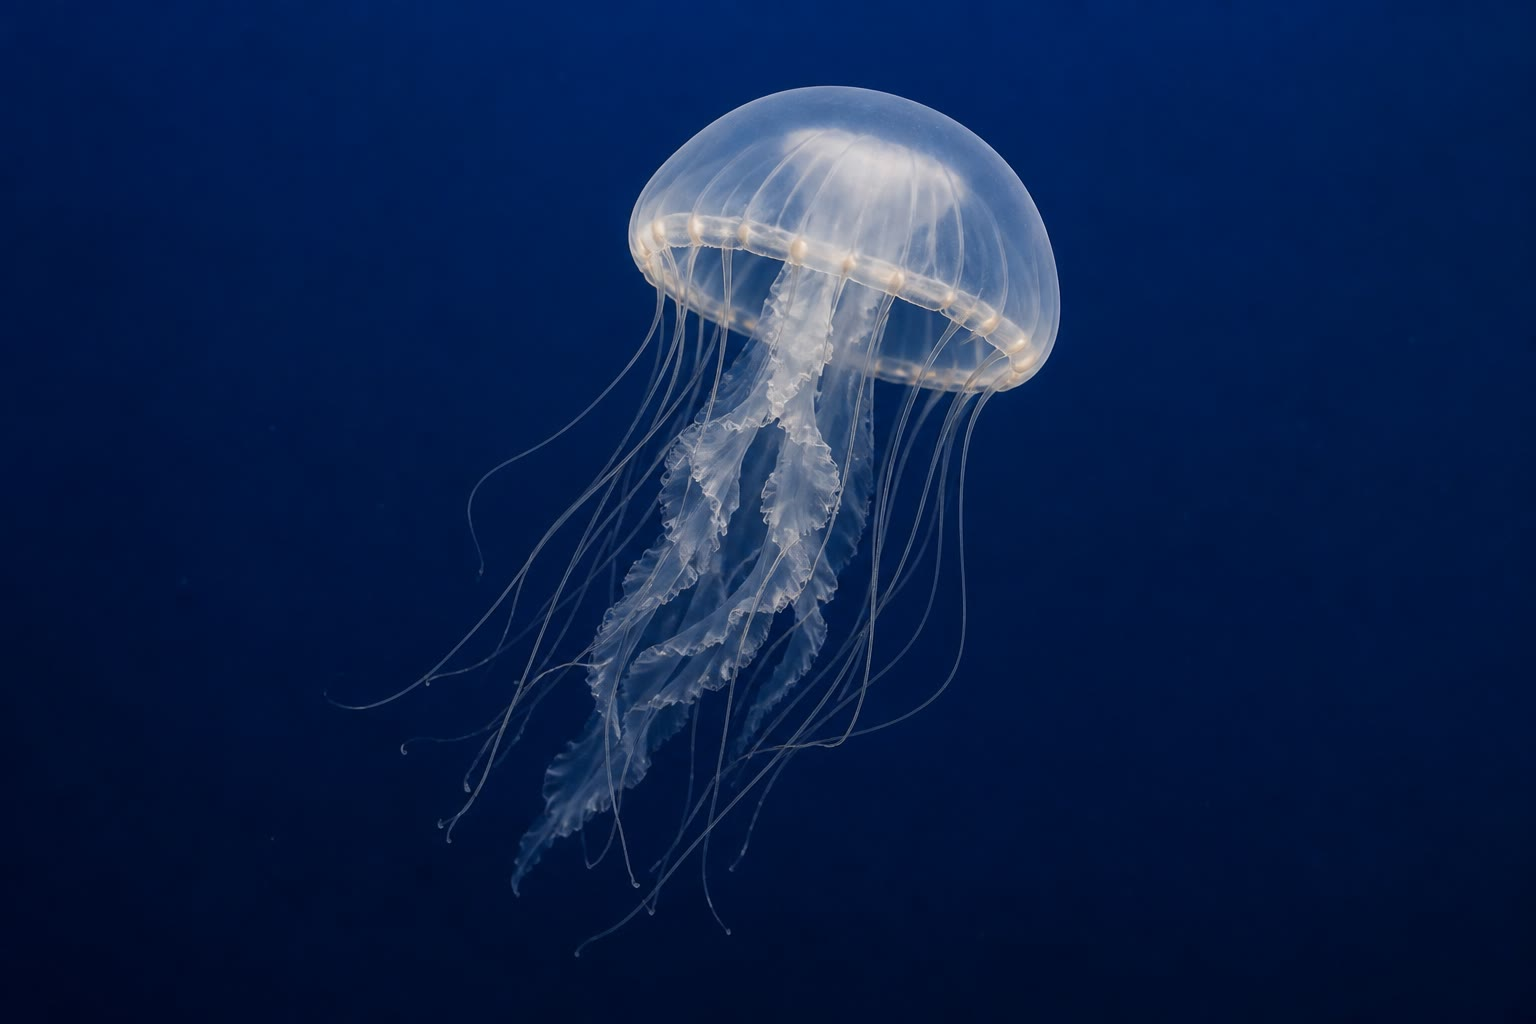
\includegraphics[width=0.46\linewidth]{images/book5/ai/b5-17-jellyfish.jpg}\hspace{0.04\linewidth}
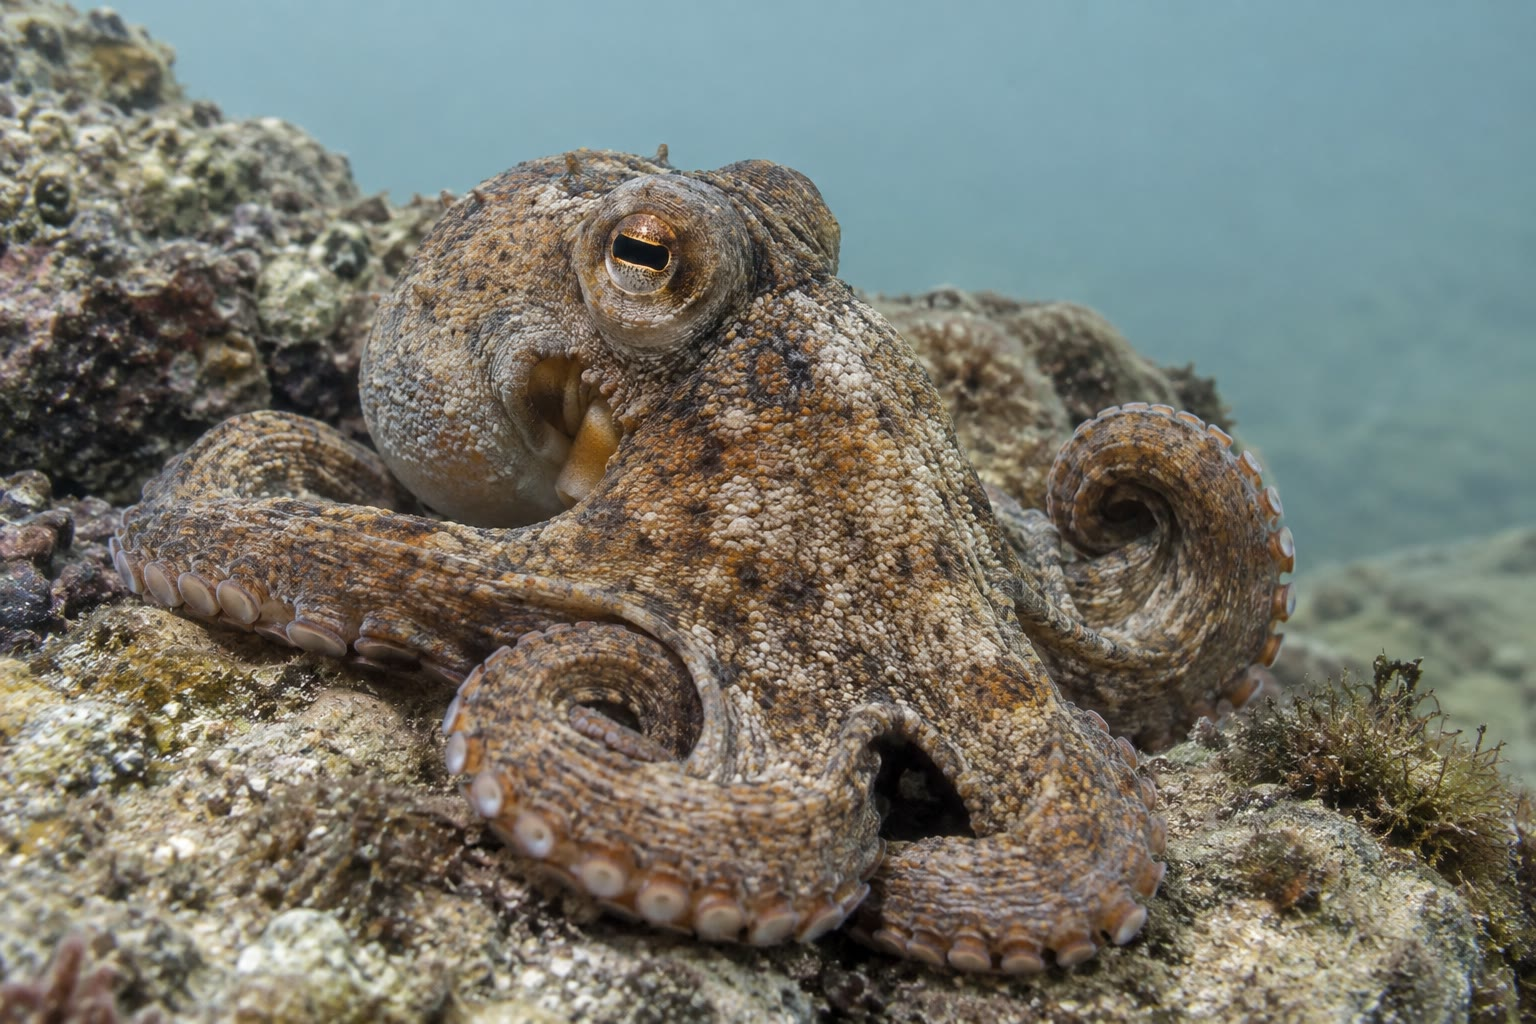
\includegraphics[width=0.46\linewidth]{images/book5/ai/b5-17-octopus.jpg}

{\small Dois modos de organizar neurônios. À esquerda: uma água-viva,
cuja \omterm{def:b3:nervous-systems:comparative}{rede nervosa} e cujos anéis marginais coordenam a natação sem
encéfalo. À direita: um polvo, com meio bilhão de neurônios, a maioria
nos braços, e o maior encéfalo de qualquer invertebrado.}
\end{omfigure}

\begin{remark}[Para que serve um sistema nervoso]\label{rem:b3:nervous-systems:for}
Plantas, fungos e esponjas não têm nenhum; um animal que se move precisa
de um, e a elaboração dos sistemas nervosos acompanha as exigências do
movimento, de sentir à distância e de prever o que virá a seguir. A
\omterm{thm:b3:nervous-systems:cable}{equação do cabo} estabelece a física --- até onde e com que rapidez um
sinal viaja para um dado diâmetro e um dado isolamento; o orçamento
energético estabelece a economia; e, dentro desses limites, os mesmos
neurônios, arranjados como redes, \omterm{def:b3:nervous-systems:comparative}{gânglios} ou um córtex, produzem a
pulsação de uma água-viva, a camuflagem de um polvo ou esta frase. Os
dois capítulos seguintes tomam a ponta de entrada e o armazenamento:
como os sentidos transformam o mundo em disparos e como as sinapses
mudam para que o mundo, uma vez encontrado, seja lembrado.
\end{remark}

\section{Exercícios}

\begin{exercise}[$\star$]\label{exo:b3:nervous-systems:1}
Nomeie os quatro tipos de \omterm{def:b3:nervous-systems:cells}{glia} e uma função de cada um, e diga quais
dois fazem \omterm{def:b3:nervous-systems:cells}{mielina} e onde.
\end{exercise}

\begin{exercise}[$\star$]\label{exo:b3:nervous-systems:2}
O que a coloração de Golgi tornou possível, o que Cajal concluiu dela e
o que Golgi concluiu? Qual estava certo, e como a questão foi decidida?
\end{exercise}

\begin{exercise}[$\star$]\label{exo:b3:nervous-systems:3}
Descreva o \omterm{def:b3:nervous-systems:circuits}{arco reflexo} patelar e explique por que ele leva apenas
\qty{30}{ms} enquanto um chute voluntário leva dez vezes mais.
\end{exercise}

\begin{exercise}[$\star$]\label{exo:b3:nervous-systems:4}
Liste os efeitos simpáticos e parassimpáticos sobre o coração, a pupila,
o intestino e as vias aéreas, e o transmissor que cada divisão usa no
alvo.
\end{exercise}

\begin{exercise}[$\star\star$]\label{exo:b3:nervous-systems:5}
Calcule a \omterm{thm:b3:nervous-systems:cable}{constante de comprimento} de um axônio de \qty{1}{\micro m} com
$R_{m}
= \qty{1e4}{\ohm.cm^2}$ e $R_{i} = \qty{100}{\ohm.cm}$, e a
fração de um sinal que resta depois de \qty{2}{mm}. Que diâmetro
dobraria $\lambda$?
\end{exercise}

\begin{exercise}[$\star\star$]\label{exo:b3:nervous-systems:6}
Um axônio sensorial de \qty{12}{\micro m} percorre \qty{1.2}{m} do dedo
do pé até a medula, e um axônio motor de \qty{15}{\micro m} faz o
caminho de volta. Com \qty{6}{m/s} por micrômetro e \qty{0.5}{ms} por
sinapse, estime a latência mínima de um reflexo espinal de retirada com
um \omterm{def:b3:nervous-systems:cells}{interneurônio}. Quanto tempo levaria com axônios amielínicos do mesmo
diâmetro a $v = 1.1\sqrt{d}$?
\end{exercise}

\begin{exercise}[$\star\star$]\label{exo:b3:nervous-systems:7}
Usando o orçamento do encéfalo da
\cref{prop:b3:nervous-systems:barrier-budget}, estime quantos ATP um
neurônio pode gastar por segundo e, se um disparo com suas sinapses
custa $2\times 10^{9}$ ATP, a frequência média de disparo que o
orçamento permite. O que isso prevê a respeito do código?
\end{exercise}

\begin{exercise}[$\star\star$]\label{exo:b3:nervous-systems:8}
Explique por que um \omterm{prop:b3:nervous-systems:cpg}{oscilador de meio-centro} precisa de cansaço (ou de
outro processo lento) para oscilar, e o que aconteceria com dois
neurônios que se inibissem mutuamente e nunca se cansassem.
\end{exercise}

\begin{exercise}[$\star\star$]\label{exo:b3:nervous-systems:9}
A \omterm{prop:b3:nervous-systems:barrier-budget}{barreira hematoencefálica} exclui a dopamina, produto da L-dopa, mas
admite a L-dopa. Explique como isso é explorado na doença de Parkinson e
por que \omterm{def:b3:adaptive-immunity:antibody}{anticorpos} contra proteínas encefálicas são difíceis de entregar.
\end{exercise}

\begin{exercise}[$\star\star\star$]\label{exo:b3:nervous-systems:10}
Deduza a forma dependente do tempo da \omterm{thm:b3:nervous-systems:cable}{equação do cabo},
$\lambda^{2}\,\partial^{2}
V/\partial x^{2} = \tau\,\partial V/\partial t + V$, somando a corrente capacitiva à corrente de membrana, e mostre que
a solução estacionária do teorema decorre dela. (Enuncie a forma;
resolvê-la não é exigido.) Por que a razão $\lambda/\tau$ é uma
velocidade?
\end{exercise}

\begin{exercise}[$\star\star\star$]\label{exo:b3:nervous-systems:11}
Um axônio gigante de lula de \qty{500}{\micro m} conduz a \qty{25}{m/s}.
Usando $v \propto \sqrt{d}$, que diâmetro de axônio amielínico seria
necessário para \qty{100}{m/s}? Calcule a área de seção transversal e
compare com o axônio mielínico de \qty{20}{\micro m} que alcança essa
velocidade. O que isso implica quanto ao número de fibras rápidas que um
nervo pode carregar e quanto à evolução da \omterm{def:b3:nervous-systems:cells}{mielina}?
\end{exercise}

\begin{exercise}[$\star\star\star$]\label{exo:b3:nervous-systems:12}
A massa encefálica escala como $M_{\text{corpo}}^{0.75}$ entre os
mamíferos. Um camundongo de \qty{30}{g} tem um encéfalo de \qty{0.4}{g}.
Preveja a massa encefálica de um mamífero de \qty{70}{kg} sobre a linha,
compare com os \qty{1350}{g} humanos e discuta por que o número de
neurônios corticais, e não a massa encefálica, é o melhor correlato da
capacidade cognitiva.
\end{exercise}

\section{Problema: Cabear um Corpo}

\begin{problem}[{Problema de fim de semana --- a fiação de um corpo
orçada em constantes de comprimento, milissegundos e watts: os números
de cabo de um dendrito e de dois axônios, a latência de um reflexo do
dedo do pé à medula e de volta, a energia que o encéfalo pode pagar por
disparo e a escala dos encéfalos entre os animais, terminando na
constante de comprimento, na latência do reflexo e na frequência média
de disparo que um encéfalo consegue custear}]
\label{pb:b3:nervous-systems:1}
Dados: $R_{m} = \qty{2e4}{\ohm.cm^2}$, $R_{i} = \qty{100}{\ohm.cm}$,
$C_{m} = \qty{1}{\micro F/cm^2}$. Velocidade mielínica de \qty{6}{m/s}
por micrômetro; amielínica $v = 1.1\sqrt{d}$ m/s com $d$ em
micrômetros; atraso sináptico de \qty{0.5}{ms}. Encéfalo: \qty{20}{W},
$8.6\times 10^{10}$ neurônios, $10^{14}$ sinapses, ATP a
\qty{50}{kJ/mol}; um disparo custa $4\times 10^{8}$ ATP e cada
transmissão sináptica, $2\times 10^{4}$ ATP; um neurônio tem \num{7000}
sinapses. Escala: $M_{\text{encéfalo}} = a\,M_{\text{corpo}}^{0.75}$, com um
camundongo de \qty{30}{g} tendo um encéfalo de \qty{0.4}{g}.

\medskip
\noindent\textbf{Parte I --- Cabos.}
\begin{enumerate}
  \item Calcule $\lambda$ para dendritos de \qty{1}{\micro m} e de
        \qty{4}{\micro m}, e $\tau$.
  \item Uma sinapse a \qty{300}{\micro m} do soma, no dendrito de
        \qty{1}{\micro m}, produz \qty{5}{mV} localmente. O que chega ao
        soma? E no dendrito de \qty{4}{\micro m}?
  \item Explique por que um neurônio pode ponderar suas entradas pelo
        lugar da árvore onde elas caem, e por que as entradas precisam
        chegar dentro de cerca de $\tau$ para se somar.
  \item Calcule a velocidade de um axônio mielínico de \qty{10}{\micro m}
        e a de um axônio amielínico do mesmo diâmetro. Que diâmetro de
        axônio amielínico igualaria o mielínico?
  \item Áreas de seção transversal do axônio de \qty{10}{\micro m} e do
        equivalente amielínico. Quantos axônios mielínicos cabem no
        espaço de um axônio amielínico equivalente?
  \item Uma doença desmielinizante retira a \omterm{def:b3:nervous-systems:cells}{mielina} de um axônio de
        \qty{10}{\micro m} ao longo de \qty{2}{cm}. Estime o atraso extra
        nesse trecho se ele conduzir como um axônio amielínico desse
        diâmetro, e diga por que a condução pode falhar por completo.
\end{enumerate}

\medskip
\noindent\textbf{Parte II --- Latências.}
\begin{enumerate}[resume]
  \item Um dedo do pé toca uma superfície quente. O axônio sensorial
        (\qty{10}{\micro m}, \qty{1.2}{m}) chega à medula, um
        \omterm{def:b3:nervous-systems:cells}{interneurônio}, e um axônio motor (\qty{15}{\micro m},
        \qty{1.1}{m}) volta à perna. Latência mínima da retirada?
  \item O sinal também sobe por um axônio de \qty{10}{\micro m} ao longo
        de \qty{0.6}{m} até o encéfalo e atravessa mais duas sinapses
        antes que a dor seja sentida. Quando a dor é sentida em relação
        à retirada?
  \item Uma fibra de dor é amielínica, de \qty{1}{\micro m}. Quanto tempo
        seu sinal leva para percorrer os \qty{1.8}{m} até o encéfalo?
        Explique as duas fases da dor de um dedo do pé batido.
  \item A perna de uma girafa é \qty{2}{m} mais longa. Recalcule a
        latência do reflexo e comente os problemas do tamanho.
  \item O reflexo patelar é monossináptico, \qty{30}{ms} num adulto.
        Usando \qty{0.8}{m} em cada sentido a \qty{80}{m/s}, uma sinapse
        e uma junção neuromuscular (\qty{1}{ms}), e \qty{5}{ms} para o
        músculo desenvolver força, explique os \qty{30}{ms}.
  \item Os axônios de um recém-nascido são amielínicos. Explique por que
        seus reflexos são lentos e seus movimentos descoordenados, e o
        que a mielinização dos dois primeiros anos muda.
\end{enumerate}

\medskip
\noindent\textbf{Parte III --- O orçamento.}
\begin{enumerate}[resume]
  \item Converta \qty{20}{W} em ATP por segundo e em ATP por neurônio
        por segundo.
  \item Um neurônio dispara um potencial: ele custa $4\times 10^{8}$ ATP
        por si e aciona \num{7000} sinapses a $2\times 10^{4}$ cada.
        Custo total de um disparo com suas consequências?
  \item Que frequência média de disparo o orçamento sustenta se tudo
        fosse gasto em disparos? E se metade for para custos de repouso?
  \item Os neurônios corticais disparam a cerca de \qty{1}{Hz} em média.
        Que fração do orçamento é isso, e o que implica sobre como a
        informação é codificada?
  \item Um encéfalo que disparasse todos os neurônios a \qty{50}{Hz}
        precisaria de quantos watts? Compare com os \qty{100}{W} do corpo
        inteiro.
  \item A glicose abastece o encéfalo a \qty{5}{g/h}. Quantos watts são
        (\qty{16}{kJ/g})? É suficiente, e o que acontece com a
        consciência segundos depois de o abastecimento falhar?
\end{enumerate}

\medskip
\noindent\textbf{Parte IV --- Escalas.}
\begin{enumerate}[resume]
  \item Encontre $a$ a partir do camundongo, depois preveja a massa
        encefálica de um mamífero de \qty{70}{kg} e de um elefante de
        \qty{5000}{kg} sobre a linha.
  \item Valores reais: humano, \qty{1350}{g}; elefante, \qty{4800}{g}.
        Calcule a razão de cada espécie em relação à previsão (o
        quociente de \omterm{def:b3:nervous-systems:comparative}{encefalização}).
  \item O encéfalo do elefante tem $2.6\times 10^{11}$ neurônios, mas
        $5.6\times 10^{9}$ no córtex; o humano, $8.6\times 10^{10}$ e
        $1.6\times 10^{10}$. Onde estão os neurônios do elefante, e o que
        isso sugere sobre o que o córtex faz?
  \item O volume de um neurônio cresce com o comprimento de seu axônio,
        de modo que encéfalos maiores têm neurônios maiores e mais
        esparsos. Explique por que dobrar a massa encefálica não dobra o
        número de neurônios, e por que os primatas, cujos neurônios
        continuam pequenos enquanto o encéfalo cresce, ganham mais
        neurônios por grama que os roedores.
  \item Um polvo tem $5\times 10^{8}$ neurônios, dois terços nos braços.
        Proponha o que um braço consegue e o que não consegue fazer sem
        o encéfalo, e um experimento para testá-lo.
  \item O nematódeo \emph{C.~elegans} tem $302$ neurônios e cerca de
        \num{7000} sinapses ao todo, todas mapeadas. Compare suas
        sinapses por neurônio com a cifra humana, e diga o que um
        diagrama completo da fiação pode e não pode nos dizer sobre o
        comportamento.
  \item Resuma: a \omterm{thm:b3:nervous-systems:cable}{constante de comprimento} do dendrito de
        \qty{1}{\micro m} (questão~1), a latência do reflexo de retirada
        (questão~7) e a frequência média de disparo que o orçamento do
        encéfalo permite com metade de sua energia em disparos
        (questão~15).
\end{enumerate}
\end{problem}
